\documentclass[12pt]{article}
\newenvironment{problem}[2][Problem]{\begin{trivlist}
\item[\hskip \labelsep {\bfseries #1}\hskip \labelsep {\bfseries #2.}]}{\end{trivlist}}
\usepackage{amssymb}
\usepackage{amsmath}
\usepackage{fancyhdr}

\usepackage{enumitem}
\usepackage{graphicx}
\usepackage{hyperref}
\usepackage{color}

\usepackage{etoolbox,refcount}
\usepackage{multicol}

\newcounter{countitems}
\newcounter{nextitemizecount}
\newcommand{\setupcountitems}{%
  \stepcounter{nextitemizecount}%
  \setcounter{countitems}{0}%
  \preto\item{\stepcounter{countitems}}%
}
\makeatletter
\newcommand{\computecountitems}{%
  \edef\@currentlabel{\number\c@countitems}%
  \label{countitems@\number\numexpr\value{nextitemizecount}-1\relax}%
}
\newcommand{\nextitemizecount}{%
  \getrefnumber{countitems@\number\c@nextitemizecount}%
}
\newcommand{\previtemizecount}{%
  \getrefnumber{countitems@\number\numexpr\value{nextitemizecount}-1\relax}%
}
\makeatother    
\newenvironment{AutoMultiColItemize}{%
\ifnumcomp{\nextitemizecount}{>}{3}{\begin{multicols}{2}}{}%
\setupcountitems\begin{itemize}}%
{\end{itemize}%
\unskip\computecountitems\ifnumcomp{\previtemizecount}{>}{3}{\end{multicols}}{}}


% \begin{itemize}
%     \item Here are two columns
%   \begin{AutoMultiColItemize}
%   \item Item 1
%   \item Item 2
%   \item Item 3
%   \item Item 4
%   \item Item 5
%   \item Item 6
%   \end{AutoMultiColItemize}
%   \item AutoMultiColItemize can be nested in an itemize
%   \item Or it does not have to be.
%   \item Normal itemize, like this one, are still single column.
% \end{itemize}
% Here is one column
% \begin{AutoMultiColItemize}
% \item Item 1
% \item Item 2
% \item Item 3
% \end{AutoMultiColItemize}


\begin{document}

\pagestyle{fancy}
\fancyhf{}
\lhead{GEOL 362A -- PS 3}
\rhead{Due: 5 Nov 2021}

% \title{Problem Set 1}
% % \author{GEOL 362A, Middlebury College}
% % \date{Due: 24 Sept 2021}
% \maketitle

\noindent The goal of this assignment is to practice interpreting information from the scientific literature, with applications to a societally relevant challenge.


\begin{problem}{1}
[2 points] Consider two glaciers with similar surface slope and average ice temperature.  One glacier is twice as thick as the other.  How much strain heating at the base would you expect for the thicker glacier compared to the thinner one?  {\em Hint: express as a ratio or multiplicative factor.}
\end{problem}


\begin{problem}{2}
[5 points] Consider the glacier temperature profiles shown in Figure \ref{fig:Aru_profiles}.  

\begin{figure}[b]
    \centering
    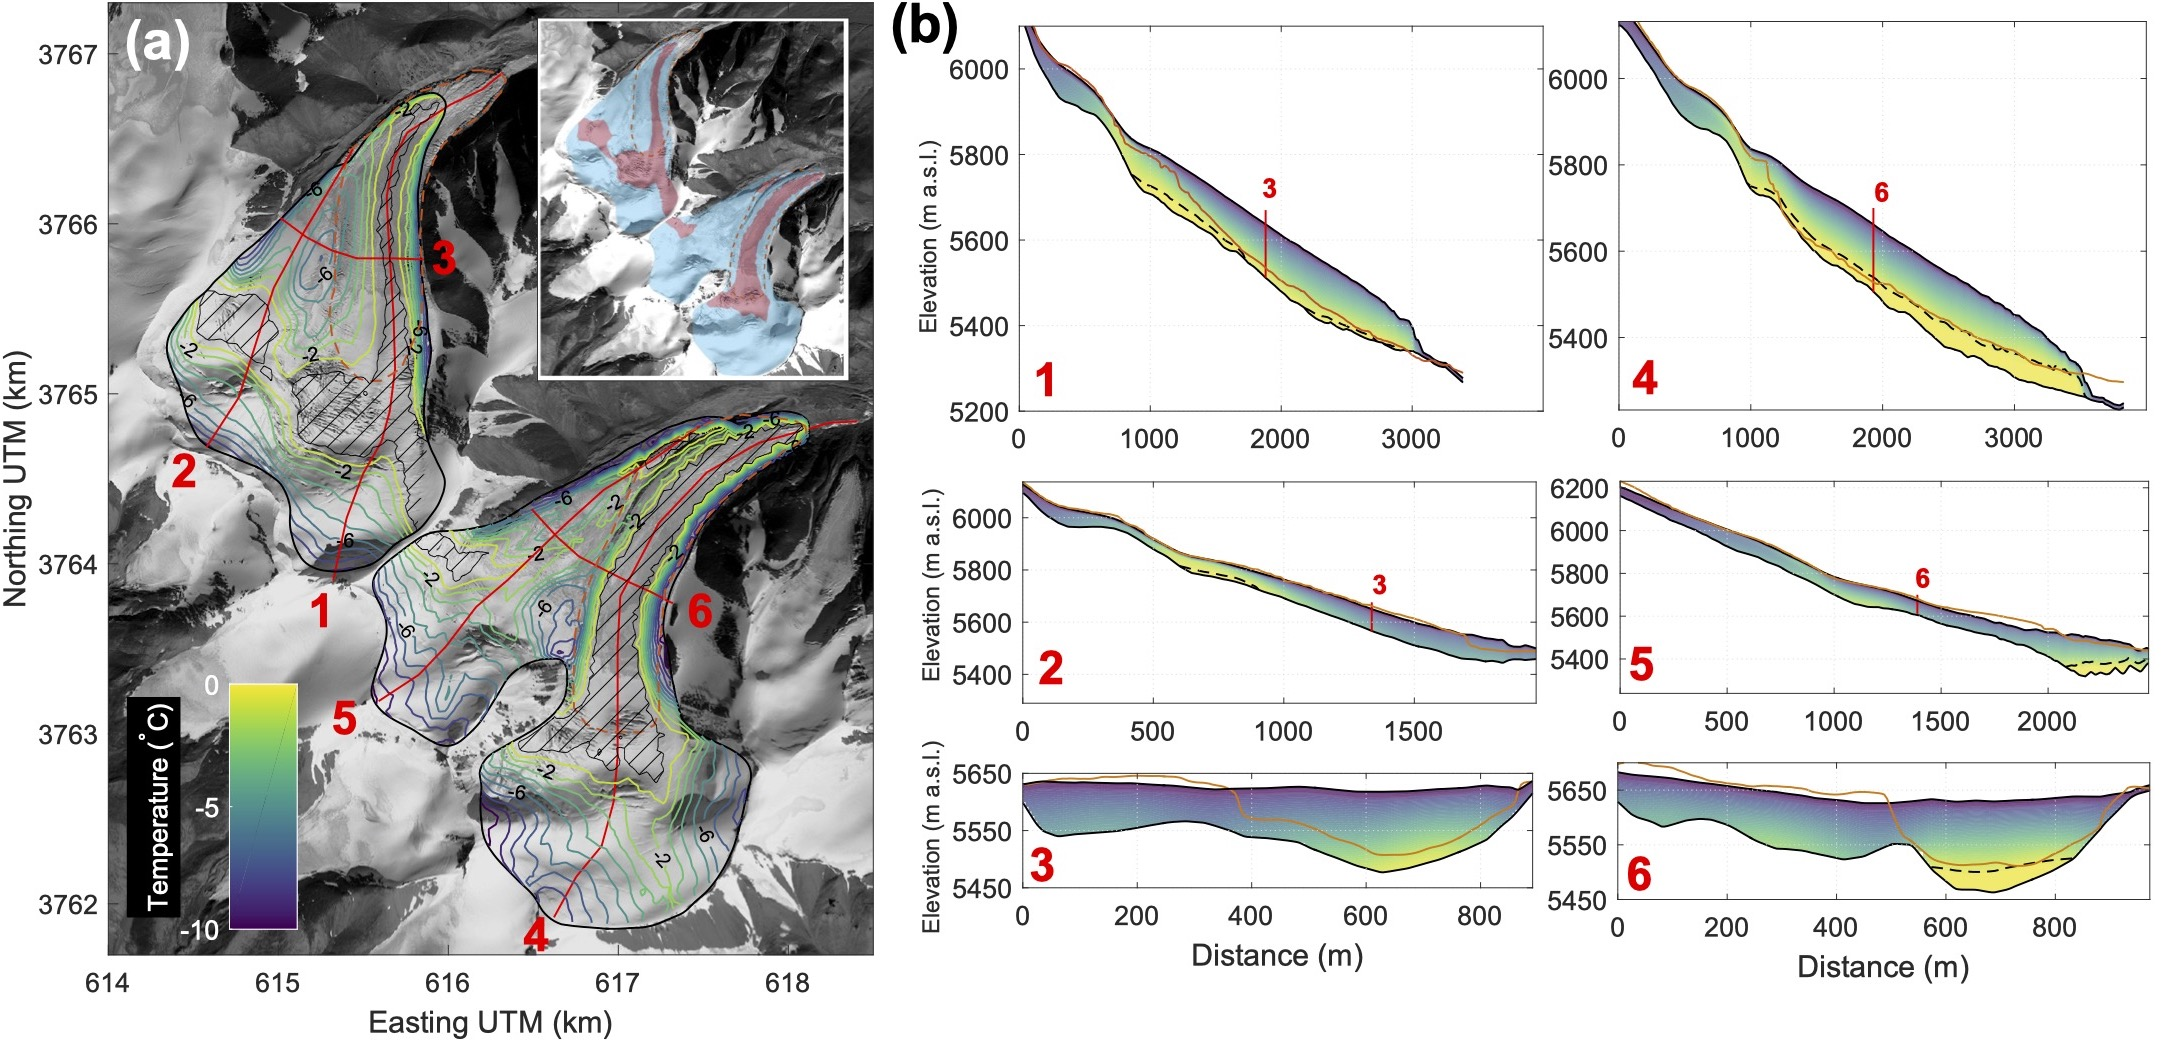
\includegraphics[width=1.0\linewidth]{figs/Figure_5b copy.jpg}
    \caption{Modelled thermal profiles of the Aru glaciers, from \href{https://tc.copernicus.org/articles/12/2883/2018/}{Gilbert et al. 2018}.  Notice that profiles (1,2) and (4,5) are pairs, each pair taken side by side on a single glacier, while profiles 3 and 6 are taken across flow.  Notice also that the horizontal scales are not consistent between the plots. \\
    Original figure caption: {\em Modelled steady-state temperature on the Aru-1 and Aru-2 glaciers. Left panel shows basal temperature with black hatched lines showing temperate areas. The inset highlights temperate-based (red) and cold-based (blue) areas. Orange dashed lines indicate the detachment outline. Panel (b) shows 2-D temperature profiles 1 to 6 as indicated in panel (a) (red lines). Profiles include Pléiades 2016 elevation profiles (orange lines). The dashed black lines indicate the cold-temperate transition surface. Note that vertical scale is exaggerated in profiles 1 and 4.}}
    \label{fig:Aru_profiles}
\end{figure}


\renewcommand{\labelenumi}{(\alph{enumi})}
\begin{enumerate}[itemsep=2pt]
   \item Describe the pattern of ice temperature along flow in profile 4.
   \item  Describe the differences you notice between along-flow temperature profiles 4 and 5.  Identify three processes or mechanisms that could be responsible for these differences.
   \item The Aru glaciers underwent catastrophic collapse in 2016, as illustrated in Figure \ref{fig:Aru_collapse}.  Figure \ref{fig:Aru_profiles}(a) shows the collapsed portions outlined in orange.  Based on this figure, your analysis, and class discussions, what factors could have contributed to the collapse?
\end{enumerate}


\begin{figure}
    \centering
    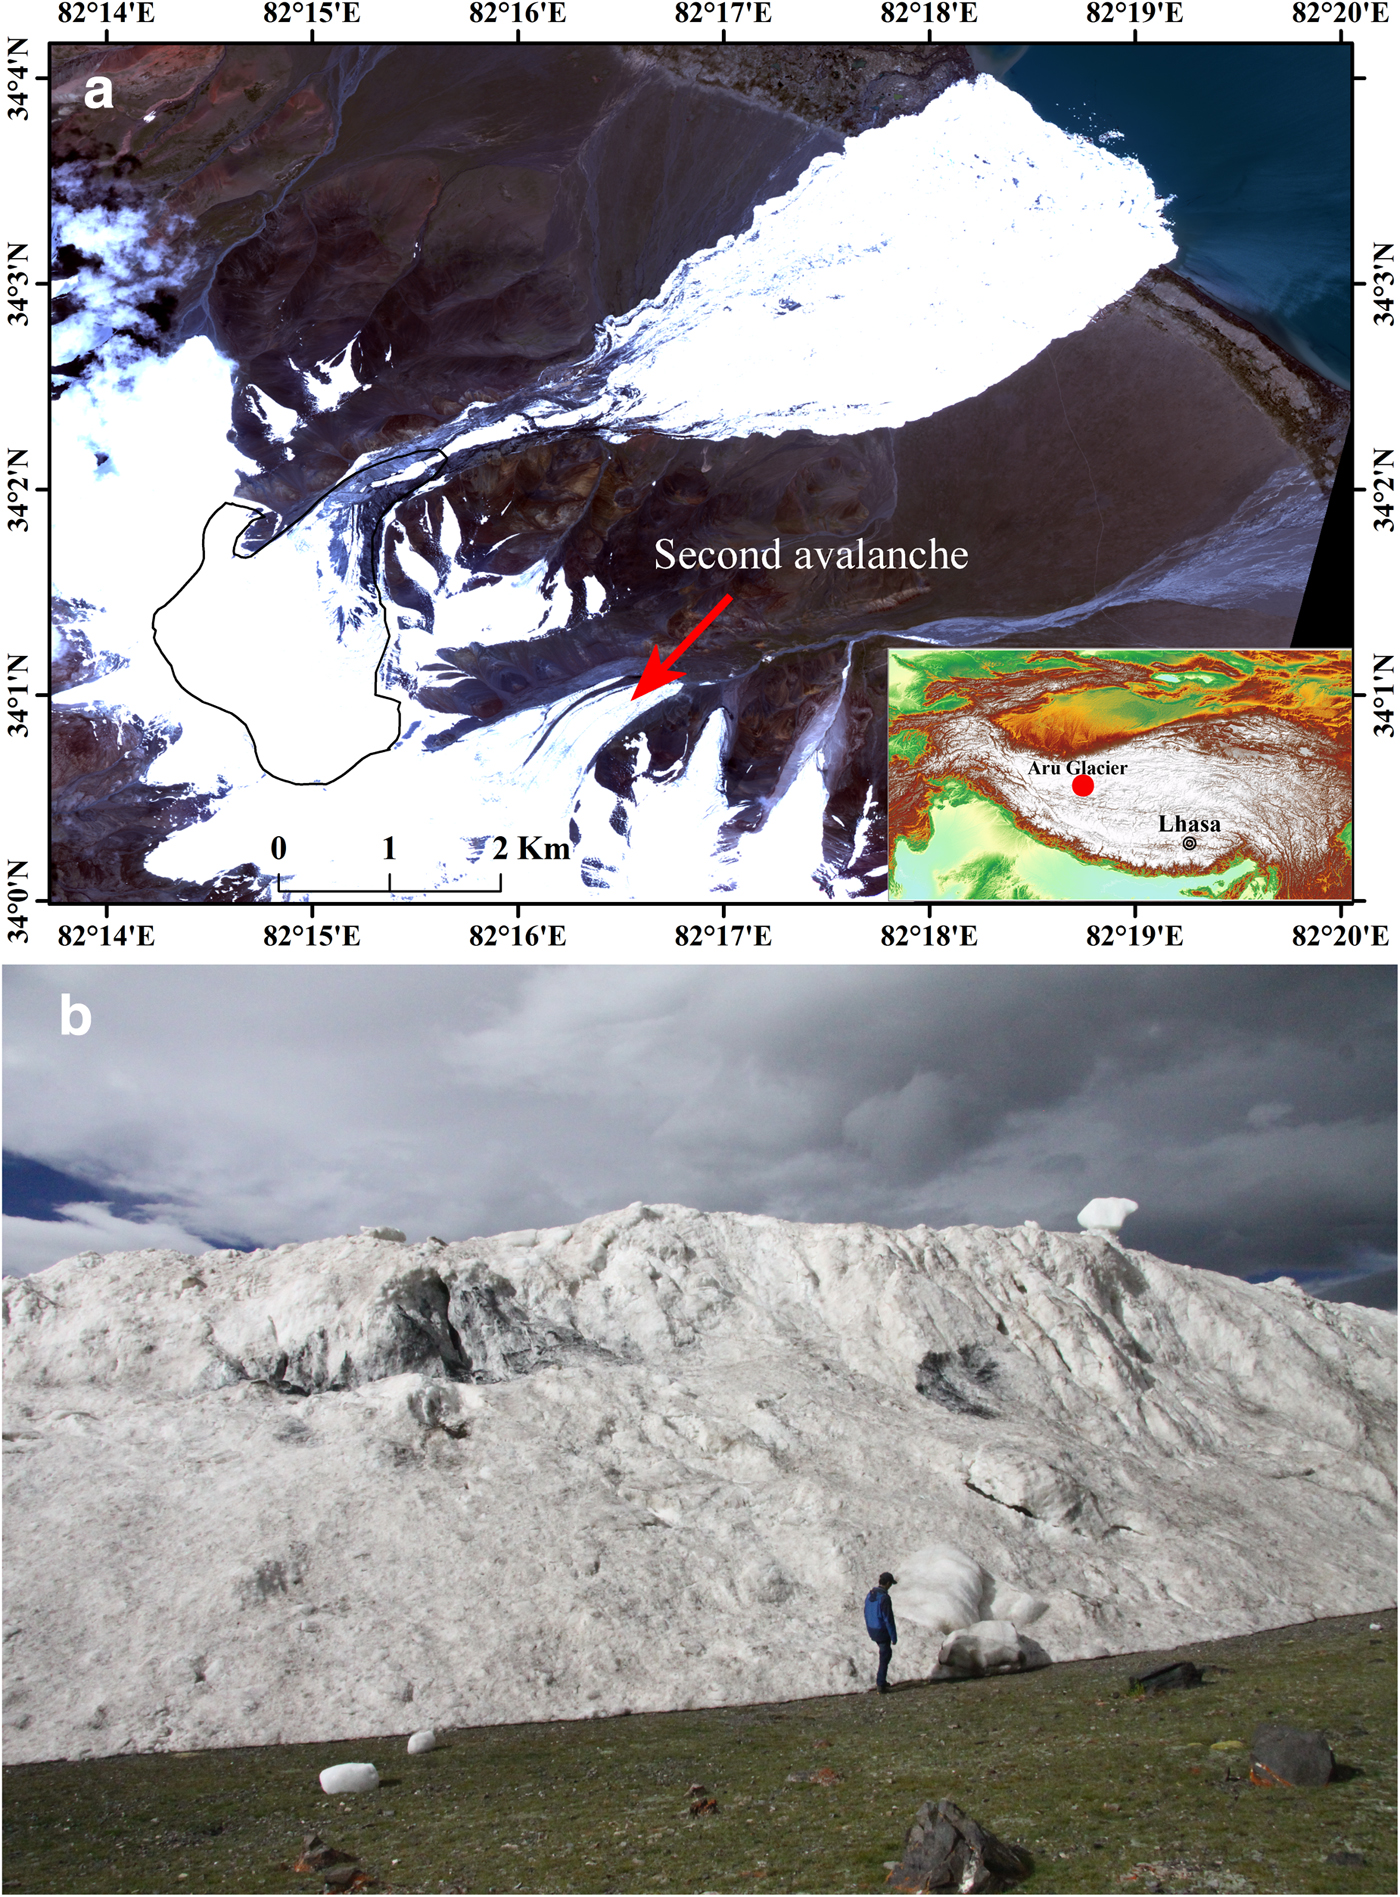
\includegraphics[width=0.7\linewidth]{figs/Tian-Figure_1.jpg}
    \caption{Satellite and in situ imagery documenting the first Aru collapse, which was followed two months later by collapse of the neighboring glacier. Figure from \href{https://www.cambridge.org/core/journals/journal-of-glaciology/article/two-glaciers-collapse-in-western-tibet/881D7526DCBCB83E45728829F13F802E}{Tian et al 2016}. Original caption: {\em The Chinese high-resolution satellite Gaofen-2 (band 321) satellite image taken on 25 July 2016. (a) Inset map shows the location of the Aru Glacier and the extent of the runout of the Aru Glacier collapse of 17 July 2016. The avalanche flowed over 6 km and reached the Aruco Lake. (b) Deposition depths exceeded 10 m.}}
    \label{fig:Aru_collapse}
\end{figure}

\end{problem}

%%%%%
\begin{problem}{3}
 [8 points]
 Catastrophic collapses such as those at Aru have only recently been observed.
 The Aru collapses killed nine herders; a comparable event on the Kolka glacier in 2002 buried the Russian village of Nizhniy Karmadon, killing at least 125 people \href{https://earthobservatory.nasa.gov/features/Kolka}{(Lindsay, 2004)}. 
 %Similar events that included impact into water have been reported in Uttarakhand, India in 2021 (destroying a dam and leaving more than 200 people missing) and Salkantay, Peru in 2020 (creating a mudflow that inundated villages near Machu Picchu).
 Warning of such events before they happen could save lives.
 Suppose that you are contracted by a mountain community to forecast local glacier collapse hazards.  
\renewcommand{\labelenumi}{(\alph{enumi})}
\begin{enumerate}[itemsep=2pt]
   \item Describe the criteria you would apply to select a numerical model for use in your forecasting.
   \item Choose two numerical models%
   \footnote{Models discussed in class include OGGM, ISSM, SICOPOLIS, HiDEM, Elmer/Ice, and ICESHEET; you may choose two of these or identify another model in the literature.}. 
   Write one to two paragraphs evaluating their suitability for this task. Identify the strengths and weaknesses of each, with citations to model documentation or  description papers.
   \item What data (for example bed topography, surface profile along/across flow, meteorological data, ...) would you seek to collect to improve your forecasting of collapse events?  You may find helpful hints in the literature, including Tian et al \href{https://www.cambridge.org/core/journals/journal-of-glaciology/article/two-glaciers-collapse-in-western-tibet/881D7526DCBCB83E45728829F13F802E}{(\textcolor{blue}{link})} and Gilbert et al \href{https://tc.copernicus.org/articles/12/2883/2018/}{(\textcolor{blue}{link})}.
  
\end{enumerate}

\end{problem}



\end{document}